\chapter{Diseño mecánico del sistema}
\ihead[]{Capítulo 5: Diseño mecánico del sistema}
\label{ch:CH05}
%%%%%%%%%%%%%%%%%%%%%%%%%%%%%%%%%%%%%%%%%%
En este capítulo se describen los elementos mecánicos empleados en la implementación del banco de pruebas. En primer lugar, se presenta el diseño de la carcasa, la cual integra los elementos de interfaz (botones, LEDs indicadores, puertos de programación y transferencia de datos) y los conectores para la alimentación y los terminales del motor bajo prueba (tipo banana). Posteriormente, se detalla la bancada de ensayos basada en perfiles de aluminio tipo V-SLOT de \(20\times 80~\mathrm{mm}\), seleccionados para estandarizar los puntos de fijación de los soportes. Finalmente, se presentan los elementos de sujeción del motor, el mecanismo de transmisión solidario al eje, incluyendo el montaje de un imán para la detección del sensor de efecto \textit{hall}, y la estructura destinada a fijar este.

En la Figura~\ref{fig:cad_general_sistema} se muestra el modelo CAD general del conjunto, a partir del cual se describen los componentes en las secciones siguientes.

\begin{figure}[H]
  \centering
  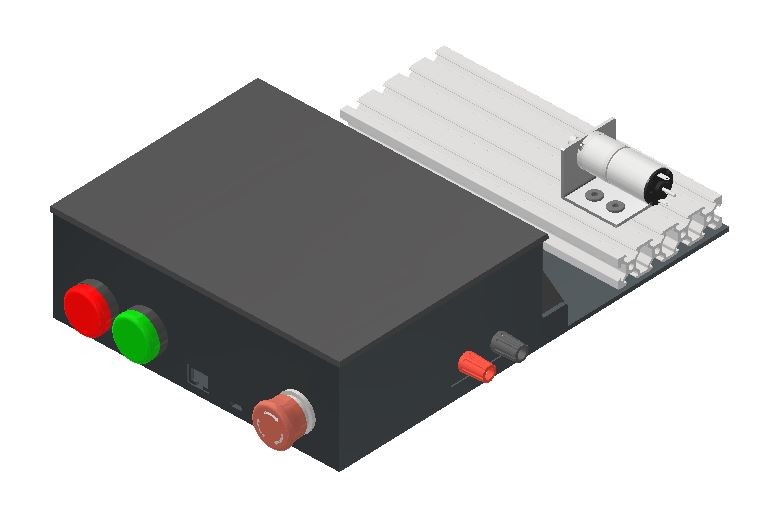
\includegraphics[width=0.92\linewidth]{CHPTRS/CH05_DIS_MECANICO/Fig/CAD1.JPG}
  \caption{Modelo CAD general del sistema mecánico del banco de pruebas.}
  \label{fig:cad_general_sistema}
\end{figure}

%============================================================
%============================================================
\section{Diseño de la carcasa y elementos de interfaz}
\label{sec:carcasa_elementos}

La carcasa del banco de pruebas se diseñó para proteger la electrónica, ordenar el cableado y centralizar los elementos de interacción del usuario durante la operación. En particular, se incorporaron alojamientos en el panel frontal para el montaje de los botones de encendido, apagado y parada de emergencia, cuyas dimensiones fueron medidas previamente en físico para asegurar un ajuste adecuado. Asimismo, se incluyeron conectores tipo banana para facilitar la conexión rápida de los terminales del motor bajo prueba y de la fuente externa de alimentación.

Estas consideraciones se ilustran en la Figura~\ref{fig:carcasa_interfaz_subfig}, donde se muestran (a) las perforaciones destinadas a los botones de control y (b) la disposición de los conectores tipo banana en el panel de conexiones.

\begin{figure}[H]
  \centering
  \begin{subfigure}[t]{0.48\textwidth}
    \centering
    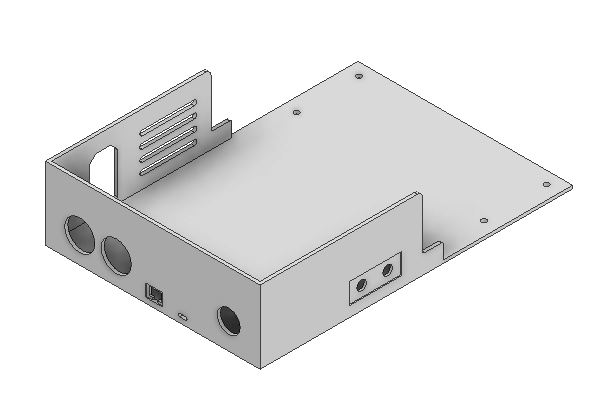
\includegraphics[width=\linewidth]{CHPTRS/CH05_DIS_MECANICO/Fig/carcasa.JPG}
    \caption{Perforaciones para botones de control y parada de emergencia.}
    \label{fig:carcasa_botones}
  \end{subfigure}
  \hfill
  \begin{subfigure}[t]{0.48\textwidth}
    \centering
    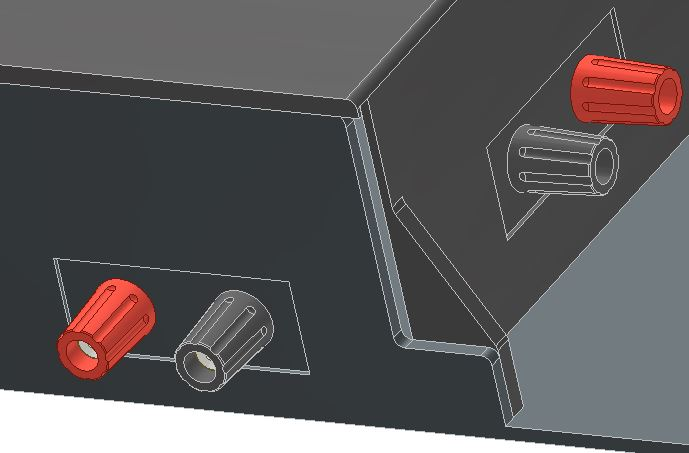
\includegraphics[width=\linewidth]{CHPTRS/CH05_DIS_MECANICO/Fig/CAD12.JPG}
    \caption{Conectores tipo banana para motor y alimentación externa.}
    \label{fig:carcasa_banana}
  \end{subfigure}
  \caption{Elementos principales de interfaz integrados en la carcasa.}
  \label{fig:carcasa_interfaz_subfig}
\end{figure}

Adicionalmente, la carcasa integra LEDs indicadores y puertos para carga de código y transferencia de datos, los cuales se presentan en la Figura~\ref{fig:carcasa_interfaz_usuario}. Estos elementos permiten supervisar el estado del sistema y habilitan la comunicación con la interfaz de usuario durante la toma de datos.

\begin{figure}[H]
  \centering
  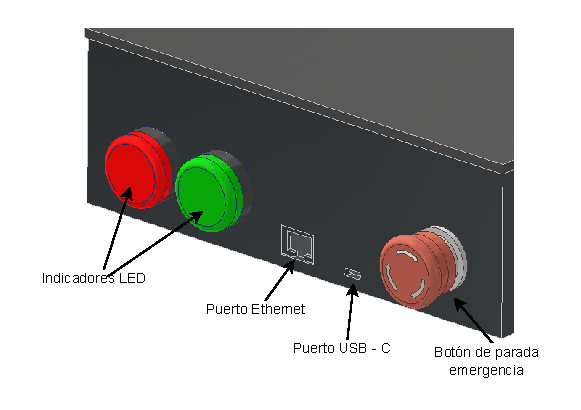
\includegraphics[width=0.85\linewidth]{CHPTRS/CH05_DIS_MECANICO/Fig/CAD10.pdf}
  \caption{Distribución de botones, LEDs indicadores y puertos de programación/datos en la carcasa.}
  \label{fig:carcasa_interfaz_usuario}
\end{figure}

Como medida adicional de protección, se incorpora un interruptor general de emergencia ubicado al inicio de la línea de alimentación del sistema. Este elemento permite el corte inmediato de energía y, además, integra un fusible para protección ante sobrecorriente, contribuyendo a resguardar el conjunto en caso de una falla eléctrica (p. ej., un cortocircuito). La disposición de este elemento se muestra en la Figura~\ref{fig:carcasa_switch_fusible}.

\begin{figure}[H]
  \centering
  % Reemplaza el nombre del archivo por el que usarás en tu tesis
  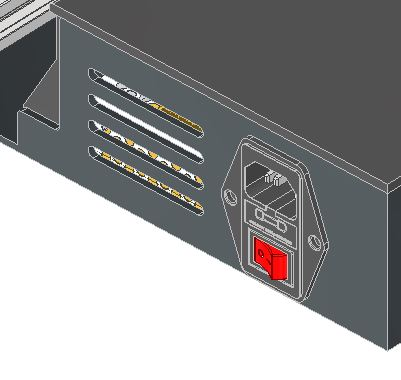
\includegraphics[width=0.55\linewidth]{CHPTRS/CH05_DIS_MECANICO/Fig/CAD11.JPG}
  \caption{Interruptor general con fusible integrado para corte y protección al inicio de la alimentación.}
  \label{fig:carcasa_switch_fusible}
\end{figure}
%============================================================


\subsection{Criterio simple de fijación carcasa--bancada}
\label{subsec:fijacion_carcasa_bancada}

La unión entre la carcasa (chapa metálica) y la bancada (perfil V-SLOT de aluminio) se realiza mediante cuatro apoyos, cada uno conformado por una unión atornillada con tuerca tipo martillo que genera presión sobre el perfil. La Figura~\ref{fig:fix_carcasa_vslot_detalle} muestra el detalle del ensamble empleado (tornillo, arandela, chapa y tuerca tipo martillo alojada en la ranura del perfil).

% ---------------------------------------------------------
% INSERTAR FIGURA: detalle de fijación carcasa--bancada
% ---------------------------------------------------------
\begin{figure}[H]
  \centering
  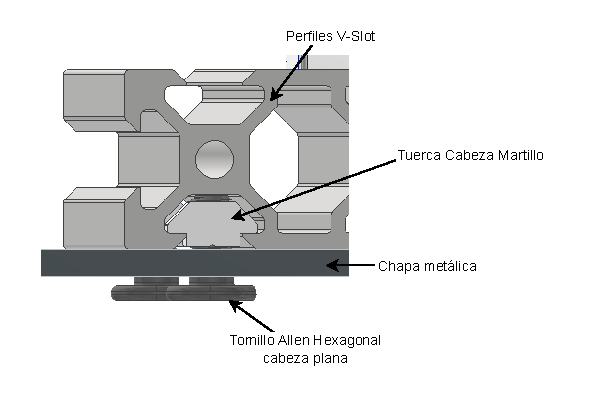
\includegraphics[width=0.6\linewidth]{CHPTRS/CH05_DIS_MECANICO/Fig/CAD8.drawio.pdf}
  \caption{Detalle de fijación carcasa--bancada mediante tornillo, arandela y tuerca tipo martillo sobre perfil V-SLOT.}
  \label{fig:fix_carcasa_vslot_detalle}
\end{figure}

Para estimar de forma preliminar la fuerza necesaria para que el conjunto deslice sobre el perfil (antes de reajustar la posición), se modela la resistencia al movimiento como fricción entre aluminio y acero (tuerca/tornillería). Para esta combinación, valores típicos reportados son \(\mu_s \approx 0.61\) (fricción estática) y \(\mu_k \approx 0.47\) (fricción cinética). \autocite{misumi_friction}

Si se considera que cada apoyo aporta una fuerza normal de apriete \(F_p\) (debida al ajuste del tornillo), la capacidad de fricción total puede aproximarse como:

\begin{align}
N_{\text{tot}} &\approx \sum_{i=1}^{4} F_{p,i} + W, \label{eq:ntot_fix}\\
F_{s,\max} &\approx \mu_s\,N_{\text{tot}}, \label{eq:fsmax_fix}\\
F_{k} &\approx \mu_k\,N_{\text{tot}}, \label{eq:fk_fix}
\end{align}

donde \(W\) es el peso total del subconjunto montado. En la práctica, cuando existe apriete, el término dominante suele ser \(\sum F_{p,i}\), por lo que \(W\) resulta secundario frente a la fuerza de sujeción.

\textit{Ejemplo numérico.} Suponiendo cuatro apoyos con un apriete moderado equivalente a \(F_{p,i}\approx 500~\mathrm{N}\) por apoyo, se obtiene \(N_{\text{tot}}\approx 2000~\mathrm{N}\) (despreciando \(W\) frente al apriete). Con ello:

\begin{align}
F_{s,\max} &\approx 0.61\,(2000)\approx 1220~\mathrm{N}, \label{eq:fsmax_num}\\
F_k &\approx 0.47\,(2000)\approx 940~\mathrm{N}. \label{eq:fk_num}
\end{align}

Este resultado respalda que, con cuatro puntos de fijación, el conjunto permanece estable ante esfuerzos de operación y vibración, y sólo deslizaría si se aplica una fuerza comparable a la indicada en la Ecuación~\eqref{eq:fsmax_num} o si se reduce el apriete. Cabe resaltar que \(\mu_s\) y \(\mu_k\) dependen del acabado superficial, limpieza y posible lubricación; por ello, estos valores se emplean como una referencia de diseño. \autocite{misumi_friction}



%============================================================
\section{Bancada de pruebas con perfiles V-SLOT}
\label{sec:bancada_vslot}

La bancada se implementa con perfiles de aluminio tipo V-SLOT de \(20\times 80~\mathrm{mm}\). Esta selección permite estandarizar los puntos de montaje mediante la ranura del perfil, facilitando el ajuste de posición de los soportes (brackets) y del conjunto del sensor. Adicionalmente, los perfiles presentan un acabado resistente y un ensamblaje práctico mediante tuercas cabeza de martillo y tornillos hexagonales de cabeza plana, lo que reduce el tiempo de reconfiguración durante pruebas con motores de geometrías distintas.

% ---------------------------------------------------------
% INSERTAR FIGURA: perfil V-SLOT 20x80 + detalle de ranura
% ---------------------------------------------------------
% \begin{figure}[H]
%   \centering
%   \includegraphics[width=0.85\linewidth]{CHPTRS/CH05_DIS_MECANICO/Fig/vslot_20x80.pdf}
%   \caption{Perfil V-SLOT de \(20\times 80~\mathrm{mm}\) empleado como bancada del banco de pruebas.}
%   \label{fig:vslot_20x80}
% \end{figure}

% ---------------------------------------------------------
% INSERTAR FIGURA: tuerca martillo + tornillo cabeza plana (detalle de sujeción)
% ---------------------------------------------------------
% \begin{figure}[H]
%   \centering
%   \includegraphics[width=0.85\linewidth]{CHPTRS/CH05_DIS_MECANICO/Fig/tnut_sujecion.pdf}
%   \caption{Sistema de fijación sobre perfil V-SLOT mediante tuerca tipo martillo y tornillería hexagonal.}
%   \label{fig:tnut_sujecion}
% \end{figure}

%============================================================
\section{Bracket de sujeción del motor y restricción de dimensiones}
\label{sec:bracket_motor}

Los brackets del motor se diseñan para sujetar el motor mediante los tornillos de su carcasa, manteniendo una fijación rígida y repetible variando unicamente los tornillos de fijación con la carcasa de los motores. Estos brackets se montan sobre la bancada V-SLOT utilizndo tuercas tipo martillo, lo que permite desplazar el motor a lo largo del perfil y ajustar su posición respecto al sensor.

Debido a la altura y geometría de la bancada (\(20\times 80~\mathrm{mm}\)), para motores de gran diámetro la sujeción puede requerir elevadores adicionales con el fin de alinear el eje del motor con el plano del sensor. En particular, conforme aumenta el diámetro del motor, aumenta la altura necesaria del bracket, reduciendo la rigidez del conjunto y aumentando la sensibilidad a vibración. Por este motivo, se establece una restricción práctica de dimensiones para los motores que se probarán, priorizando motores cuyos diámetros permitan el alineamiento sin incrementos excesivos de altura sobre la bancada.

% ---------------------------------------------------------
% INSERTAR FIGURA: bracket del motor montado sobre V-SLOT (vista CAD y/o foto)
% ---------------------------------------------------------
% \begin{figure}[H]
%   \centering
%   \includegraphics[width=0.85\linewidth]{CHPTRS/CH05_DIS_MECANICO/Fig/bracket_motor_vslot.pdf}
%   \caption{Bracket de sujeción del motor fijado sobre la bancada V-SLOT.}
%   \label{fig:bracket_motor_vslot}
% \end{figure}

%============================================================
\section{Mecanismo de transmisión y acople solidario al eje}
\label{sec:mecanismo_transmision}

Para transmitir el giro del eje hacia el conjunto de sensado se emplea un acople de geometría simple inspirado en bujes comerciales, diseñado para montarse solidario al eje y asegurar la repetibilidad del montaje. Esta solución permite escalar la geometría del acople a distintos diámetros de eje, manteniendo el mismo principio de fijación mediante tornillo prisionero.

En este trabajo se consideran ejes de \(4~\mathrm{mm}\) y \(6~\mathrm{mm}\), por lo que se diseñan variantes del acople con el diámetro interno correspondiente. Con el fin de estandarizar la tornillería del conjunto, el acople y el soporte del imán se preparan para roscas M3, empleando un macho para generar la rosca durante el prototipado. Además, dado que la estimación de parámetros requiere considerar la inercia total acoplada al eje, se priorizan geometrías compactas que minimicen masa adicional.

\begin{figure}[H]
    \centering
    \begin{tabularx}{\linewidth}{>{\centering\arraybackslash}X}
        \begin{subfigure}[t]{0.55\linewidth}
            \centering
            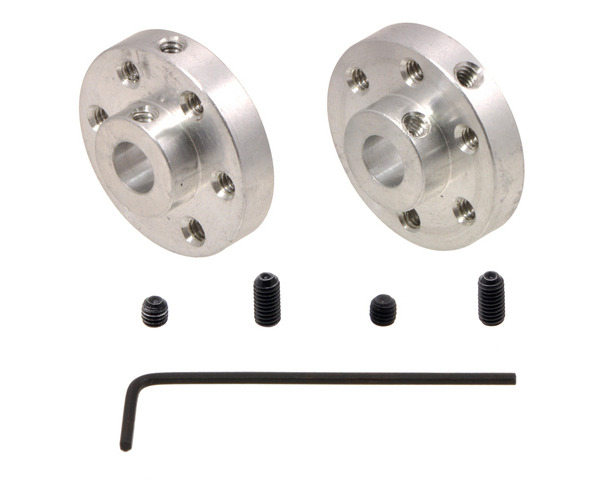
\includegraphics[width=\linewidth]{CHPTRS/CH03_DICON/Fig/CH03_FIG03_SolucionOptima/04a_SO_MotorPololu1.jpg}
        \end{subfigure}
    \end{tabularx}
    \caption{Bujes de fijación referenciales (inspiración para el acople del eje).}
    \label{fig:bujes_referenciales}
\end{figure}

% ---------------------------------------------------------
% INSERTAR FIGURA: acople para eje 4 mm y 6 mm (dos vistas)
% ---------------------------------------------------------
\begin{figure}[H]
  \centering
  \begin{subfigure}[t]{0.48\textwidth}
    \centering
    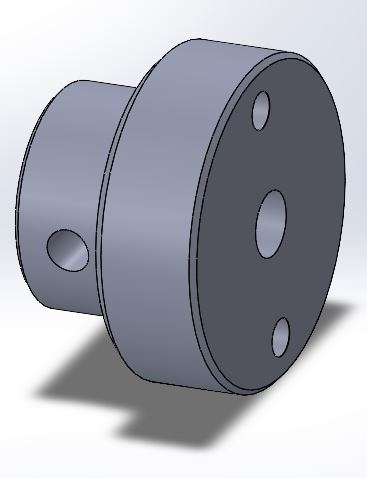
\includegraphics[width=0.65\linewidth]{CHPTRS/CH05_DIS_MECANICO/Fig/01a_AcopleIman.JPG}
    \caption{Acople para eje de 4 mm.}
    \label{fig:acople_4mm}
  \end{subfigure}
  \hfill
  \begin{subfigure}[t]{0.48\textwidth}
    \centering
    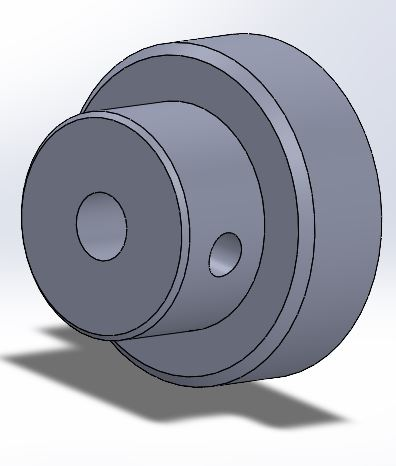
\includegraphics[width=0.65\linewidth]{CHPTRS/CH05_DIS_MECANICO/Fig/01b_AcopleIman.JPG}
    \caption{Acople para eje de 6 mm.}
    \label{fig:acople_6mm}
  \end{subfigure}
  \caption{Variantes del acople para distintos diámetros de eje.}
  \label{fig:acoples_eje}
\end{figure}

El acople incluye puntos de fijación para un soporte destinado a posicionar el imán de neodimio de forma concéntrica con el eje. 
% La Figura~\ref{fig:soporte_iman_acople} muestra la pieza diseñada para fijarse al acople y alojar el imán, manteniéndolo expuesto y próximo al sensor.

% \begin{figure}[H]
%   \centering
%   \begin{tabularx}{\linewidth}{>{\centering\arraybackslash}X}
%     \begin{subfigure}[t]{0.60\linewidth}
%       \centering
%       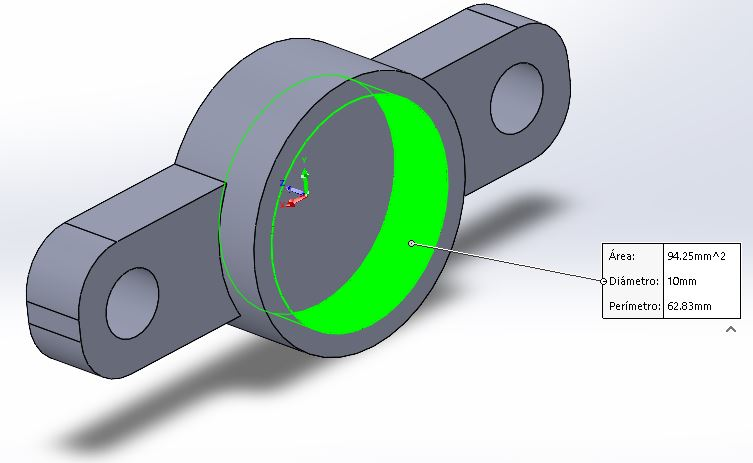
\includegraphics[width=\linewidth]{CHPTRS/CH05_DIS_MECANICO/Fig/02_SoporteIman.JPG}
%     \end{subfigure}
%   \end{tabularx}
%   \caption{Soporte de imán diseñado para fijarse al acople solidario al eje.}
%   \label{fig:soporte_iman_acople}
% \end{figure}

\begin{figure}[H]
  \centering
  \begin{tabularx}{\linewidth}{>{\centering\arraybackslash}X}
    \begin{subfigure}[t]{0.55\linewidth}
      \centering
      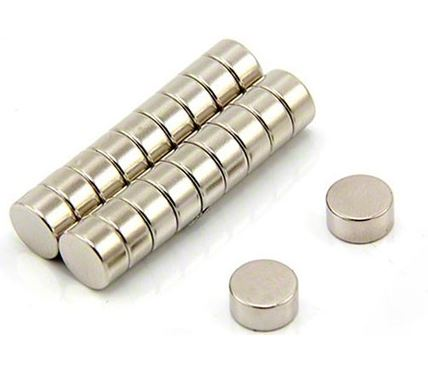
\includegraphics[width=\linewidth]{CHPTRS/CH05_DIS_MECANICO/Fig/CAD9.JPG}
    \end{subfigure}
  \end{tabularx}
  \caption{Imán de neodimio seleccionado para las pruebas (diámetro nominal \(5~\mathrm{mm}\)).}
  \label{fig:iman_neodimio}
\end{figure}

Para la etapa de prototipado y validación, estas piezas se fabrican mediante impresión 3D y se evalúan en el Capítulo~\ref{ch:CH07}. Para la solución final, se considera emplear un material no magnético, como por ejemplo, aluminio, con el fin de no alterar el campo del imán durante el sensado.

%============================================================
\section{Estructura de fijación del sensor de efecto \textit{hall}}
\label{sec:estructura_sensor_hall}

El sensado de posición angular y velocidad angular se realiza mediante el integrado TMAG5170. Para garantizar mediciones consistentes, la \ac{PCB} del sensor debe fijarse sobre una estructura rígida que permita ubicar el sednsor TMAG5170 de manera coaxial con el eje del motor. Adicionalmente, se busca que el conjunto sea simétrico respecto a la bancada, de modo que el eje del motor pueda posicionarse centrado y el sensado se realice en condiciones geométricas repetibles.

\subsection{Principio de funcionamiento y criterio de alineamiento}
\label{subsec:funcionamiento_tmag}

El TMAG5170 estima el ángulo a partir de la variación del campo magnético en el plano \(XY\). Por ello, se emplea un imán de neodimio polarizado montado solidario al eje del motor, de modo que la orientación magnética varíe con el giro. En la Figura~\ref{fig:tmag_magnet_setup} se presenta un esquema de referencia para el montaje del imán y, adicionalmente, la ubicación de la zona activa del sensor dentro del integrado, la cual se utiliza como referencia para el alineamiento.

\begin{figure}[H]
\centering
\begin{subfigure}[t]{0.48\textwidth}
    \centering
    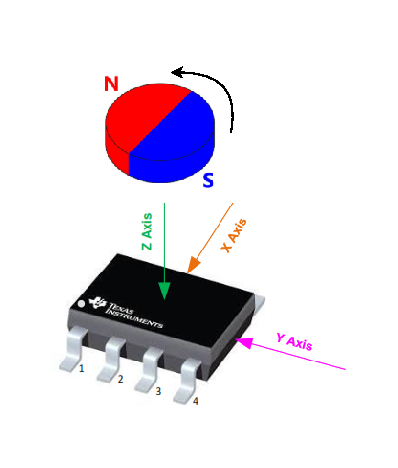
\includegraphics[width=\linewidth]{CHPTRS/CH05_DIS_MECANICO/Fig/CAD6.pdf}
    \caption{Esquema de referencia para el montaje del imán respecto al sensor.}
    \label{fig:tmag_magnet_scheme}
\end{subfigure}
\hfill
\begin{subfigure}[t]{0.48\textwidth}
    \centering
    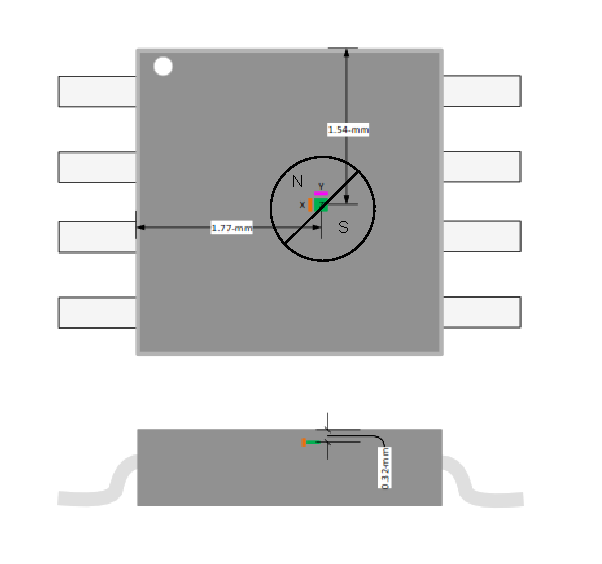
\includegraphics[width=\linewidth]{CHPTRS/CH05_DIS_MECANICO/Fig/CAD7.pdf}
    \caption{Ubicación aproximada de la zona activa del sensor de efecto \textit{hall} en el integrado.}
    \label{fig:tmag_hall_location}
\end{subfigure}
\caption{Referencia de montaje del imán y ubicación del sensor en el TMAG5170.}
\label{fig:tmag_magnet_setup}
\end{figure}

\subsection{Selección del imán}
\label{subsec:seleccion_iman_mec}

Con base en las pruebas documentadas en el Capítulo~\ref{ch:CH07}, se evaluaron imanes de distintos tamaños para mejorar la estabilidad del sensado. Considerando que el TMAG5170 tiene dimensiones reducidas (del orden de \(3~\mathrm{mm}\times 3~\mathrm{mm}\)), se observó que imanes muy grandes incrementan la sensibilidad a desalineamientos y pueden degradar la coherencia de la medición. En contraste, el imán de \(5~\mathrm{mm}\) de diámetro presentó un desempeño más estable, al facilitar el alineamiento del conjunto imán--sensor y mejorar la repetibilidad de la estimación de ángulo.

% ---------------------------------------------------------
% INSERTAR FIGURA: soporte completo PCB sensor + ajuste de distancia al imán (vista CAD)
% ---------------------------------------------------------
% \begin{figure}[H]
%   \centering
%   \includegraphics[width=0.85\linewidth]{CHPTRS/CH05_DIS_MECANICO/Fig/soporte_pcb_sensor.pdf}
%   \caption{Estructura de fijación de la \ac{PCB} del TMAG5170 y referencia de su alineamiento coaxial con el eje del motor.}
%   \label{fig:soporte_pcb_sensor}
% \end{figure}

%============================================================
% Nota para ti (no es parte del texto final si no quieres):
% Figuras sugeridas por sección (para que las consigas):
% - Carcasa: CAD del panel frontal, detalle LEDs/puertos, conectores banana, distribución interna.
% - Bancada V-SLOT: perfil 20x80, tuerca martillo + tornillo, vista de montaje sobre bancada.
% - Brackets: bracket montado, ejemplo motor pequeño vs motor grande (comparativa de altura).
% - Transmisión: acoples 4 mm y 6 mm, soporte del imán, imán real.
% - Sensor hall: soporte de PCB, esquema de coaxialidad, referencia de distancia imán--sensor.
%============================================================
